\documentclass[conference]{IEEEtran}
\usepackage{cite}
\usepackage{graphicx}
\usepackage{multirow}

% correct bad hyphenation here
\hyphenation{op-tical net-works semi-conduc-tor}


\newcommand{\toolName}{OUR TOOL}

\begin{document}
%
% paper title
% Titles are generally capitalized except for words such as a, an, and, as,
% at, but, by, for, in, nor, of, on, or, the, to and up, which are usually
% not capitalized unless they are the first or last word of the title.
% Linebreaks \\ can be used within to get better formatting as desired.
% Do not put math or special symbols in the title.
\title{\toolName: Navigating Program Flow in the IDE}


% author names and affiliations
% use a multiple column layout for up to three different
% affiliations
\author{\IEEEauthorblockN{Chris Brown, Justin Smith, Tyler Albert, and Emerson Murphy-Hill}
\IEEEauthorblockA{Department of Computer Science\\
North Carolina State University\\
Raleigh, North Carolina 27606\\
Email: \{dcbrow10, jssmit11, tralber2\}@ncsu.edu, emerson@csc.ncsu.edu}
}

% make the title area
\maketitle

% As a general rule, do not put math, special symbols or citations
% in the abstract
\begin{abstract}
Program navigation is a critical task for software developers. 
Unfortunately, the current state-of-the-art tools do not adequately support developers in simultaneously navigating both control flow and data flow (i.e. program flow). 
To assist developers in effectively navigating program flow we designed and implemented a tool that leverages powerful program analysis techniques while maintaining low barriers to invocation.
Our tool enables developers to systematically navigate program flow upstream and downstream within the Eclipse IDE.
Based on a preliminary evaluation with 8 participants, our tool compares well to existing tools. 
%Something about tradeoffs.
%For simple sub-tasks tool was effective with very few interface elements. 
\end{abstract}

% no keywords



\IEEEpeerreviewmaketitle


\section{Introduction}
%Probably need to add in the minimalist angle. How much can we achieve with minimal alterations to the IDE.
%Existing tools feature many cumbersome UI widgets or seem poorly integrated into the IDE.
%
Modern software systems contain millions of lines of source code. 
As software grows in size and complexity, developers increasingly rely on tools to help them navigate the programs they create. 
Program navigation is a central task tied to many critical activities, including exploring new code bases, debugging, and assessing security vulnerabilities. 

While navigating programs, developers ask questions about control flow and data flow throughout the program~\cite{latoza2010hard, Smith2015}. We will refer to these two concepts together as \textit{program flow}. Developers are interested in navigating program flow to trace how data is modified across multiple method invocations.

Integrated development environments (IDEs) present code linearly in the order methods are defined. However, successful developers do not navigate source code linearly (line by line starting at the top of the file). Instead, they methodically navigate the code's hierarchical semantic structures~\cite{robillard2004investigate}. To resolve this conflict and realize their ideal navigation strategies, developers rely on program navigation tools. 

% Much work has focused on helping developers visualize and navigate call graphs,
% we also interested in 
% Probably more to come in here? What are some current tools and why are they limited.
% Discuss program visualization tools vs navigation tools.

In this work we will design, implement, and evaluate a program navigation tool.
To address the limitations of existing program navigation tools, our tool will embody five key design principles (Section \ref{DesignPrinciples}). We will implement our tool as a plugin to the Eclipse IDE. 

This paper makes the following contributions:


\section{Background}
Summary of related work, including a table evaluating existing tools on various design principles.
Spoiler alert, none of the tools satisfy all of the principles.


\section{Design Principles and Implementation}
\label{DesignPrinciples}
In this section we describe the design principles that we used to shape \toolName. We derived these design principles by evaluating the limitations of existing program navigation tools.
 
\vspace{1em} 
\noindent\textbf{Powerful Program Analysis -}
By leveraging powerful program analysis techniques, navigation tools can provide more accurate information.
For example, by analyzing abstract syntax trees (ASTs) and call graphs, tools can make proper references to variables and methods. 
Simple textual analysis may lead to inaccurate results, especially when programs include inheritance and duplicate variable names.

\vspace{1em} 
\noindent\textbf{Low Barriers to Invocation -}
Barriers to invocation may inhibit adoption. 
As developers may wish to navigate multiple program paths concurrently, repetitively invoking the tool may be cumbersome, especially if barriers are high. 


\vspace{1em} 
\noindent\textbf{Full Program Navigation -}
Developers are not only interested in traversing programs' call graph, but also how data flows through the call graph.
To do so, developers must inspect the relationship between methods as well as the methods themselves.
Often the methods of interest span across multiple source files.
Furthermore, program navigation tools should support this traversal both upstream and downstream. 
That is, tools should highlight variable assignments and also subsequent variable uses. 

\vspace{1em} 
\noindent\textbf{In Situ Results -}
Switching between views in the IDE can cause disorientation~\cite{deAlwis2006disorient}. As developers navigate through code, navigation tools should present their results in that context. 
When navigation tools present results outside the code, developers are burdened with the cognitive load of translating those results back to the code.



\section{\toolName}
We implemented \toolName~as a plugin to the Eclipse IDE~\cite{Eclipse}. We chose Eclipse because of its popularity and extensibility. 
Eclipse is one of the most widely used open source IDEs for Java development and it provides many extension points for plugins. Figure \ref{fig:tool} depicts our tool...

\begin{figure*}
	\centering
	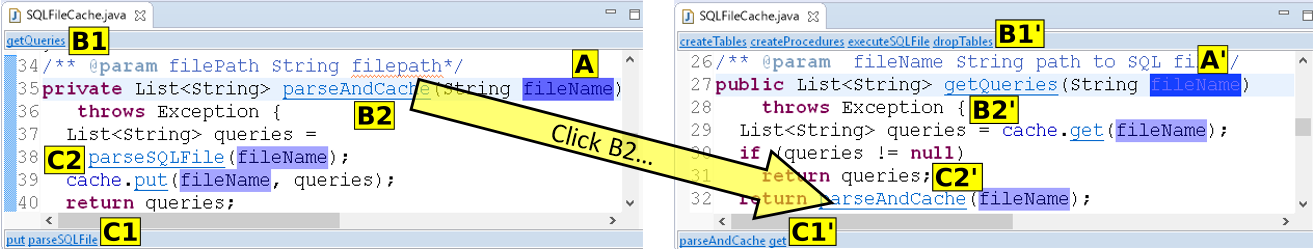
\includegraphics[width=\textwidth]{images/toolScreenshot}
	\caption{(A) - When a user clicks on a variable all (visible) instances of that variable are highlighted in the code. (B) - When the variable has been declared as a parameter to the current method, users can click on that method's name in the editor to navigate to a location where that method is called. (X) - When the variable is passed to an external method, users can click on that method's name to open its declaration. (C) - If the variable is passed in from another method or is defined earlier in the current file, a link to that location is displayed in the ``top box.'' (D) - If the variable is passed in to another method or referenced later in the current file, links to those locations appear in the ``bottom box.''}
	\label{fig:tool} 
\end{figure*}

%TODO- Update image and description for B/C 1/2

\begin{table}
\centering
\caption{Participant Demographics}
\begin{tabular}{|c|c|c|c|}
%\rowcolor{gray!50}
\hline
Participant & Industry & Java &\multicolumn{1}{c|}{Previous} \\
%\rowcolor{gray!50}
& Experience (years) & Experience (years) & \multicolumn{1}{c|}{Eclipse Use} \\
\hline
P1 & 9 & 5 & Yes \\
\hline
P2 & 0 & 6 & Yes \\
\hline
P3 & 3 & 2 & No \\
\hline
P4 & 5 & 0 & No \\
\hline
P5 & 12 & 10 & Yes \\
\hline
P6 & 0 & 3.5 & Yes \\
\hline
P7 & 1 & 9 & Yes \\
\hline
P8 & 5.5 & 3.5 & Yes \\
\hline
\end{tabular}
\label{table:participants}
\end{table}

\section{Preliminary Evaluation}

Pre-study questionnaire to balance Eclipse novices across groups.

2x2 latin square design


\subsection{Tasks}
We will ask developers to perform two tasks that involve program flow navigation (Task 1 and Task 3 from \cite{Smith2015}).

\subsection{Participants}
We performed a preliminary evaluation of \toolName~with eight participants.
All participants were graduate students at the time of the study and on average had 5 years of professional programming experience. 
Our goals are to get some initial feedback on the usability of our tool and evaluate whether our approach shows promise in enabling developers to efficiently navigate program flow. 

\subsection{Usability Evaluation}
To evaluate the usability of \toolName, we administered an adapted version of the Post-Study System Usability Questionnaire (PSSUQ)~\cite{Lewis95ibmcomputer}. We modified the questionnaire by replacing ``this system'' with ``this tool'' and asked questions from the System Quality and Interface Quality categories. We asked 10 questions; participants responded on a 7-point Likert scale from ``Strongly Disagree'' to ``Strongly Agree.'' 	
We also asked participants open-ended questions based on applicable categories from Nielsen's usability heuristics~\cite{Nielsen1992}

To capture participant's experiences that these two approaches overlooked, two of the authors independently examined each audio/video recording 

\section{Results}
\subsection{Quant stuff...}
Graph with average time to complete each task split by tool and no tool different colors.
Time to first method for Task 1 split by tool and no tool.

Time to first method

Correctness

\subsection{Qualitative Results} 
Satisfied with easy to use	and Simple to use and Easy to learn Participants responded positively
-Low barriers to invocation

Responded low for complete tasks quickly (performance issues and disorientation)
All the functions I expected (Missing tracability and mark bars, ... )

With our tool: Task 1 Faster than other tool, less correct. Task 2 slower, but more correct. 


\section{Discussion - Scenarios}
List scenarios when our tool worked and when it didn't
\subsection{Wins}
Getting started. Low barriers to invocation
\\
\textbf{Linear Naviagtion}
When participants navigated linearly in one direction (as in Task 1). Our tool was most effective. 
Few branches



\subsection{Losses}
Why were they slower and less accurate with our tool?
Second task: 
Lots of confounding variables.
Requires more knowledge about iTrust. Even though we signposted all the areas that (required) knowledge about iTrust...

Using our tool for task 1, everyone located a hard-coded string. But the two participants that answered incorrectly (misinterreted the information)

\subsection{Systematic Evaluation}
Program navigation tools should help developers keep track of where they have been and where they are going. Especially while attempting to resolve complex defects, developers may want to thoroughly explore all program paths. Their navigation tools should help them keep track of their progress.

\subsection{Design Implications}

Participants were taken to new locations but couldn't backtrack.
	Back buttons exist, but most didn't use and they didn't help the person who did use them...
	Points to an inherent limitation of our minimalistic approach. People would be more oriented with a graph or more persistent breadcrumbs...
Overwhelmed when the call graph had a high branching factor.
	Participants quickly navigated up single paths as in Task 1
	When call paths branched in many directions our tool could reccomend more full featured tools.
Couldn't keep track of where they had been.
	See systematic evaluation. Links could turn purple and get moved to the end of the list.
Performance.
	Whenever the user clicks on a new variable \toolName~ has to search through the entire project for locations where the method is declared or invoked. We observed that participants navigated within one file more often than between files. To improve the performance of our tool, we could optimize the search to return local results before returning global search results.
	
	They also clicked on the same variables (we could do some caching)


\section{Limitations}

\section{Conclusion}

\section*{Acknowledgment}

The authors would like to thank...





% trigger a \newpage just before the given reference
% number - used to balance the columns on the last page
% adjust value as needed - may need to be readjusted if
% the document is modified later
%\IEEEtriggeratref{8}
% The "triggered" command can be changed if desired:
%\IEEEtriggercmd{\enlargethispage{-5in}}

% references section

% can use a bibliography generated by BibTeX as a .bbl file
% BibTeX documentation can be easily obtained at:
% http://mirror.ctan.org/biblio/bibtex/contrib/doc/
% The IEEEtran BibTeX style support page is at:
% http://www.michaelshell.org/tex/ieeetran/bibtex/
\bibliographystyle{IEEEtran}
% argument is your BibTeX string definitions and bibliography database(s)
\bibliography{progNavPaper}




% that's all folks
\end{document}


